\chapter{Realisierung}
% Dies ist das Hauptkapitel Ihrer Arbeit! Hier wird die Umsetzung der eigenen Ideen und Konzepte
% (Kapitel 3) anhand der gewählten Methoden (Kapitel 4) beschrieben, inkl. der dabei aufgetretenen
% Schwierigkeiten und Einschränkungen.

Wie im Kapitel \ref{vorgehen} Vorgehensmodell beschrieben, wurde die Arbeit während mehreren Sprints realisiert.
In den folgenden Abschnitten wird das Vorgehen während er einzelnen Sprints aufgezeigt.
Dabei werden die bearbeiteten User Stories beschrieben, Entscheidungen und Designs dokumentiert sowie aufgetretene Schwierigkeiten gezeigt.
Die sechs Sprints sowie die Vorbereitungsphase fanden während folgenden Zeiten statt:

\begin{itemize}
   \item Vorbereitungsphase 14.02. - 27.02.
   \item Sprint 1 18.02. - 13.03.
   \item Sprint 2 14.03. - 27.03.
   \item Sprint 3 28.03. - 10.04.
   \item Sprint 4 11.04. - 24.04.
   \item Sprint 5 25.04. - 08.05.
   \item Sprint 6 09.05. - 22.05.
\end{itemize}

\section{Vorbereitungsphase}
Die Arbeiten am Projekt begannen mit der Vorbereitungsphase. Das Ziel dieser war es, wichtige Abklärungen zu machen und Entscheidungen zu treffen, damit im ersten Sprint mit der eigentlichen Entwicklung begonnen werden konnte.
Dies beinhaltete zum einen eine Befragung potenzieller Benutzer der zu entwickelnden Applikation sowie die Evaluation eines geeigneten Technologiestacks.
Mit einer Dauer von zwei Wochen war die Vorbereitungsphase gleich lang wie ein Sprint.
Bei ihr handelt es sich jedoch nicht um einen richtigen Sprint, da noch kein Backlog mit User Stories vorhanden ist.
Der Backlog für die Sprints wurde während dieser Phase basierend auf den Erkenntnissen der zuvor genannten Punkte erstellt.
In den folgenden Abschnitten wird die Umsetzung der Vorbereitungsphase detailliert beschrieben.

\subsection{DlmsQuickAccess}
Für die Erstellung des Projekts in \ac{ADO}, für das Git-Repository sowie für die C\# Solution wurden jeweils Namen benötigt.
Dazu wurde \textit{DlmsQuickAccess} kreiert.
Der Name ist an die zu ersetzende Funktion des \ac{DMT2}, \textit{Quick Access}, angelehnt.

\subsection{Kennenlernen der Nutzer}\label{survey}
Wie im Kapitel \ref{erwarteteResultate} erklärt, ist das Ziel dieses Projekts, eine Funktion der Software \ac{DMT2} durch eine Neuentwicklung zu ersetzen.

Am Standort Cham der Landis+Gyr gibt es zwei Entwicklerteams, welche den \ac{DMT2} regelmässig verwenden.
Für dieses Projekt wurden die Mitglieder dieser beiden Teams als Nutzer definiert.
Um die Nutzer besser kennen zu lernen, wurden die Methoden \textit{Fokusgruppe} (\ref{fokusgruppe}) und \textit{Befragung} (\ref{befragung}) eingesetzt.

Zu Beginn der Vorbereitungsphase wurden alle Nutzer zu einer Gruppendiskussion eingeladen, um eine Fokusgruppe zu bilden.
In dieser Diskussion wurden erörtert, welche Dinge bei der bestehende Anwendung bereits gut funktionieren und welche als störend wahrgenommen werden.
Ebenfalls wurde von den Nutzern Ideen \& Wünsche für die Neuentwicklung abgeholt.

Für das Sammeln der Antworten wurde während der Diskussion retrotool.io \footnote{https://retrotool.io/8mWyxCzpbIfQPydp2FPf4} eingesetzt.
Die Abbildungen \ref{fig:WhatWorksWell}, \ref{fig:WhatBothersYou} und \ref{fig:IdeasAndWishes} sind Screenshots daraus.


\begin{figure}[H]
   \centering
   \includegraphics[width=1.0\textwidth]{gfx/S1_RetroBoard_WhatWorksWell.png}
   \caption{
       Antworten der Nutzer zur Frage "Was funktioniert bereits gut?"
   }
   \label{fig:WhatWorksWell}
\end{figure}

\begin{figure}[H]
   \centering
   \includegraphics[width=1.0\textwidth]{gfx/S1_RetroBoard_WhatBothersYou.png}
   \caption{
       Antworten der Nutzer zur Frage "Was stört dich?"
   }
   \label{fig:WhatBothersYou}
\end{figure}

\begin{figure}[H]
   \centering
   \includegraphics[width=1.0\textwidth]{gfx/S1_RetroBoard_IdeasAndWishes.png}
   \caption{
       Ideen und Wünsche der Nutzer an die neue Anwendung
   }
   \label{fig:IdeasAndWishes}
\end{figure}
Anschliessend an diese Diskussion in der Fokusgruppe wurde eine Befragung mithilfe einer Online-Umfrage durchgeführt.
Das Ziel dieser war es, quantitative Daten zu erheben.
Die Resultate der Umfrage sind dieser Arbeit im Anhang \ref{anhang:survey} beigelegt.
Um herauszufinden, an welchen Funktionen als erstes gearbeitet werden soll, mussten die Nutzer zehn mögliche Features, welche auf den in der Fokusgruppe gesammelten Ideen \& Wünsche basieren, priorisieren.
In Abbildung \ref{fig:FeaturesPrio} ist das Resultat dieser Priorisierung dargestellt.

\begin{figure}[H]
   \centering
   \includegraphics[width=1.0\textwidth]{gfx/S1_Survey_Prio.png}
   \caption{
       Resultat der Umfrage: Sortiere diese Features nach Priorität
   }
   \label{fig:FeaturesPrio}
\end{figure}

Die Nutzer wurden ebenfalls dazu befragt, auf welchen Plattformen sie die neue Anwendung gerne einsetzten würden.
Im nächsten Abschnitt werden die Antworten (Abbildung \ref{fig:SurveryPlatforms}) auf diese Frage sowie viele weitere Aspekte für die Evaluation des Technologiestacks verwendet.

\begin{figure}[H]
   \centering
   \includegraphics[width=1.0\textwidth]{gfx/S0_Survey_Platform.png}
   \caption{
       Resultat der Umfrage: Gewünschte Plattformen
   }
   \label{fig:SurveryPlatforms}
\end{figure}

\subsection{Evaluation des Technologiestacks}
Um im ersten Sprint mit der Implementation der Applikation beginnen zu können, musste zuerst ein geeigneter Technologiestack evaluiert werden.
Die im vorherigen Abschnitt erwähnte Umfrage hat ergeben, dass sich alle Befragten Windows als Zielplatform der neuen Anwendung wünschen.
Nur vereinzelt wurde nebst Windows noch Android oder Linux angegeben.

Im Projektauftrag (Anhang \ref{anhang:aufgabenstellung}) ist festgehalten, dass die Technologien frei gewählt werden können, für die Landis+Gyr jedoch günstig zu unterhalten sein soll.

Um dies zu erreichen, wurden für die Evaluation nur Programmiersprachen in Betracht gezogen, welche bei der Landis+Gyr bereits aktiv verwendet werden.
Im Kapitel \ref{lgintern} werden einige Anwendungen und Softwareprojekte der Landis+Gyr, welche im Umfeld der zu entwickelnden Anwendung betrieben und unterhalten werden, genauer beschrieben.
Die dort verwendeten Programmiersprachen sind C\#, Python und C++.


Ein wichtiger Teil der Anwendung wird die \ac{DLMS} Kommunikation mit den Stromzählern sein.
Diese ist in allen drei zuvor genannten Programmiersprachen bereits implementieren und wird in den Tools \textit{\ac{ATS}}, \textit{libpydlms} rsp. \textit{\ac{DMT2}} verwendet.
Da der \ac{DMT2} jedoch von einem externen Lieferanten entwickelt wurde, erlaubt die zugehörige Lizenz die Verwendung des Codes nicht ohne Weiteres.


Der Fokus der zu entwickelnden Anwendung liegt auf der Benutzerschnittstelle.
Python-Applikationen mit Benutzerschnittstelle gibt es bei der Landis+Gyr keine.
Möglich wäre ein Technologiestack bestehend aus Python Backend mit einem Angular \footnote{https://angular.io} Frontend.
Das Web-Framework Angular, welches mit der Sprache TypeScript verwendet wird, setzt die Landis+Gyr bereits im Projekt \textit{Test Script Manager} ein.
Dieses Projekt wird an einem Standort ausserhalb der Schweiz entwickelt.
Als Backend wird dort jedoch nicht Python sondern C\# eingesetzt.
Eine Python+Angular Stack wäre somit neu für die Landis+Gyr, die einzelnen Technologien jedoch bereits etabliert.

Im Gegensatz zu Python existieren bei der Landis+Gyr bereits mehrere C\# Anwendungen, welche über eine Benutzerschnittstelle verfügen.
\textit{PicParted} und \textit{DocTool} sind C\# Anwendungen, welche eine \ac{WPF}\footnote{https://docs.microsoft.com/en-us/visualstudio/designers/getting-started-with-wpf?view=vs-2022} Benutzerschnittstelle haben.
Sie werde im Bereich des Picasso Projekts (\ref{picasso}) eingesetzt und unterhalten. 
Ursprünglich wurden sie vom Autor dieser Arbeit entwickelt.

Die Anwendung \ac{ATS}, welche im Abschnitt \ref{ats} genauer beschrieben wird, verfügt über C\# Code für die \ac{DLMS} Kommunikation mit Stromzählern.
Dieser könnte für die neue Anwendung wiederverwendet werden.
Die in Abschnitt \ref{objectModelsClassDescriptions} beschriebenen Tools verfügen ebenfalls über C\# Code, welcher thematisch nahe an der neuen Anwendung ist und eventuell ebenfalls wiederverwendet werden kann.

Aufgrund der genannten Umstände fiel die Entscheidung auf einen C\# Technologiestack.
Ein weiterer Vorteil von C\# ist, dass die Sprache, wie in Abschnitt \ref{typing} erwähnt, über eine statische sowie dynamische Typenüberprüfung verfügt.

Zur Benutzerschnittstelle gibt der Projektauftrag vor, dass diese modern und benutzerfreundlich daherkommt.
Um mit C\# Benutzerschnittstellen zu erstellen, gibt es verschiedene Frameworks.
Wie bereits erwähnt, unterhält die Landis+Gyr bereits einige Anwendungen welche mit dem Framework \ac{WPF} umgesetzt wurden.
Für die zu entwickelnde Anwendungen wurde WinUI3 als Framework gewählt.
In der Bedienung ist WinUI3 nahe an \ac{WPF} da ebenfalls das \ac{MVVM}-Muster verwendet wird und die Controls in XAML deklariert werden.
Es bietet jedoch den Vorteil, dass es das Fluent Design System von Microsoft befolgt und im Gegensatz zu \ac{WPF} noch aktiv weiterentwickelt wird.
Somit ist WinUI3 optisch und technisch moderner als \ac{WPF}.

Um im ersten Sprint direkt mit der Entwicklung loslegen zu können, wurde in \ac{ADO} ein Repository erstellt.
Dieses wurde mit einem leeren WinUI3 Projekt initialisiert.


\subsection{Erstellung des Backlogs}
Wie in Abschnitt \ref{methoden:ADO} erklärt, wird \ac{ADO} für die Verwaltung des Backlogs verwendet.
Dazu musste als erstes eine neues \ac{ADO} Projekt erstellt und die Sprints eingetragen werden.
Danach konnten User Stories formuliert und auf die sechs geplanten Sprints verteilt werden.
Welche Stories im ersten Sprint bearbeitet wurden und wie dies genau ablief, ist im folgenden Kapitel zu lesen.

\newpage

\section{Sprint 1}
Im ersten Sprint wurde der Grundstein für das Projekt sowie die Applikation gelegt.
Dies beinhaltete folgende Stories:
\begin{itemize}
   \item Teile des \ac{ATS} Codes sollen übernommen werden, so dass die Kommunikation mit Stromzählern möglich ist.
% in ADO gibt es no eine zweite story zur kommunikation, diese wird hier weggelassen
   \item Die Applikation DlmsQuickAccess soll an Benutzer soll so an Benutzer ausgeliefert werden, dass diese automatisch neue Updates erhalten.
   \item Die Applikation soll auf \ac{ADO} bei jedem neuem Commit automatisch gebaut und getestet werden. 
   \item Es soll eine Benutzerschnittstelle erstellt werden, welche alle Objekte eines Zählers auflistet.
% in ADO gibt es eine extra story zum ObjectModel parsen, diese wird hier weggelassen
\end{itemize}
In den folgenden Abschnitten werden die genannten Stories einzeln ausführlich beschrieben.
Als erstes wird jeweils das Ziel der Story genauer festgehalten.
Darauf folgen wird beschrieben wie die Story bearbeitet wurde, welche Schwierigkeiten aufgetreten sind und in welchem Zustand sich die Story zum Ende des Sprints befand.

\subsection{Implementation der Kommunikation mittels ATS Code}\label{s1:ats}
\dq Teile des \ac{ATS} Codes sollen übernommen werden, so dass die Kommunikation mit Stromzählern möglich ist.\dq

\subsubsection{Ziel}
Nebst des Codes für die Kommunikation mit Stromzähler beinhaltet das Projekt des \ac{ATS} viele weitere Komponenten wie beispielsweise eine Benutzerschnittstelle für das Verwalten von Testscripts oder einen Interpreter für die eigene Scriptsprache.
Die Story gilt als erledigt, wenn die eine erfolgreiche Kommunikation mit einem Stromzähler durchgeführt werden kann.
Dabei soll nur jener Code, welche effektiv für die Kommunikation zuständig ist, in die DlmsQuickAccess Solution eingebunden werden. 


\subsubsection{Vorgehen und Schwierigkeiten}
Als erstes wurde der ATS Code analysiert.
Dabei zeigte sich, dass alle Klassen des \ac{ATS} in einem einzelnen C\# Projekt mit dem Namen \textit{Befehlsinterpreter} abgelegt sind.
Nebst den benötigten \ac{DLMS} Kommunikationskomponenten beinhaltet dieses Projekt auch Code für Benutzerschnittstellen sowie diversen andere Kommunikationsprotokolle.
Eine saubere Trennung der einzelnen Komponenten ist nicht erkennbar. 
Dies bestätigen auch die Code Metrics Results (TODO footnote was diese sind und wie sie erstellt werden können) sichtbar in Abbildung TODO.
Einzelne Klassen sind mit bis zu 71 anderen gekoppelt, während laut \parencite{quantitativeInvestigationRiskCodeMetrics} TODO neun eine gute Obergrenze wäre.
Abbildung TODO zeigt des weiteren, dass teils englische und teils deutsche Klassennamen verwendet werden.
Es ist somit nicht möglich, den \ac{ATS} Code als Bibliothek mittels eines NuGet TODO Paketes einzubinden.
Im Kapitel \ref{ausblick:ats_split} wird jedoch darauf hingewiesen, dass es in der Zukunft sinnvoll sein könnte,
das Befehlsinterpreter Projekt aufzuspalten und einzelne Komponenten als Bibliothek bereitzustellen.

Das Aufräumen der \ac{ATS} Projekts nicht teil dieser Arbeit sein soll, wurde versucht, nur jene Teile des Codes einzubinden, welche tatsächlich gebraucht werden.
So wurde das Repository des \ac{ATS} mittels Git Subtree TODO in das DlmsQuickAccess Repository eingebunden. 
Dies ermöglichte es, dass Klassen und Funktionen, welche nicht benötigt werden, entfernt werden konnten.
Die Änderungen am \ac{ATS} Code mussten lediglich in das Repository dieser Arbeit gepusht werden.
Wäre anstelle von Git Subtree Git Submodule verwendet worden, wäre dies nicht möglich gewesen.
Neue Versionen des \ac{ATS} Code können ebenfalls gepullt und gemerget werden. 
Der Nachteil dieses Ansatzes ist es, dass es etwas schwieriger ist, die gemachten Änderungen zum Ursprungsrepository zu pushen \parencite{gitSubtree}.
Da die geplanten Änderungen jedoch nur das Löschen von Code beinhalten, ist dieser Nachteil nicht relevant.

Die Klasse \textit{ReaderWriter} wurde geschrieben, um den Zugriff auf den \ac{ATS} Code an einem Ort zu bündeln.
Diese kümmert sich um das laden benötigter Konfigurationen, initialisiert die \ac{DLMS} Kommunikation und bietet eine Methoden zum Lesen und Schrieben von Daten an, welche von der Applikation benutzt werden kann.
\begin{figure}[H]
   \centering
   \includegraphics[width=0.5\textwidth]{gfx/readerwriter.png}
   \caption{
      Unvollständiges Klassendiagramm zur ReaderWriter Klasse
      }
      \label{fig:readerwriter}
\end{figure}
Sie ist im Klassendiagramm \ref{fig:readerwriter} abgebildet.
Die Kompositionen zu \textit{CBefehl} und \textit{CKommunikation} zeigen die Abhängigkeit zum \ac{ATS} Code.


% TODO schreiben wie der Stand ende S1 aussah

\subsection{Deployment}
\dq Die Applikation DlmsQuickAccess soll an Benutzer soll so an Benutzer ausgeliefert werden, dass diese automatisch neue Updates erhalten.\dq

\subsubsection{Ziel}
Obwohl die Anwendung zu diesem Zeitpunkt noch über keinerlei Funktionen verfügt, welche für einen Benutzer nützlich sein könnten, soll das Deployment der Applikation bearbeitete werden.
Damit wird sichergestellt, dass WinUI3 Applikationen in der Umgebung der Landis+Gyr korrekt ausgeliefert werden können.
Dies ist wichtig, da es in der Vergangenheit Probleme mit restriktiven Sicherheitsrichtlinien gab.

Die Story gilt als abgeschlossen wenn es für einen Benutzer möglich ist die Applikation eigenständig zu installieren.
Updates, welche nach dem Installationszeitpunkt erscheinen, sollen automatisch aufgespielt werden.

\subsubsection{Vorgehen und Schwierigkeiten}
Da die Anwendung nur intern bei der Landis+Gyr verwendet werden wird und somit nicht über eine offizielle Quelle verteilt werden, muss sie via Sideloading installiert werden \parencite{sideload}.
Die Entwicklungsumgebung Visual Studio 2022 Enterprise, welche für die Entwicklung der Anwendung verwendet wurde, ermöglicht es Packages fürs Sideloading zu erstellen.
Über einen Dialog werden dabei Konfigurationen wie Versionsnummer, Ausgabepfad oder Prozessorarchitektur angegeben.
Die Anwendung soll auf einem Netzwerkverzeichnis abgelegt werden, auf welches alle Entwickler Zugriff haben.
Dieses wir auch für die Verteilung andere Programme wie beispielsweise der Compiler der Firmware verwendet.

Eine erste, leere Version des DlmsQuickAccess konnte einfach gebaut und über die beschriebene Funktion von Visual Studio auf das Netzwerkverzeichnis deployt werden.
Die dabei erstellte Datei \textit{DlmsQuickAccess (Package).appinstaller} konnte auf dem Rechner des Entwicklers problemlos ausgeführt und die Anwendung somit installiert werden.
Nach der ersten erfolgreichen Installation wurde eine zweite Version veröffentlicht, um zu testen, dass sich die Anwendung automatisch aktualisiert.
Dies funktioniert so, dass der DlmsQuickAccess beim jedem Start überprüft, ob sich auf dem Netzwerkverzeichnis eine neue Version befindet.
Falls dies so ist wird diese heruntergeladen und beim nächsten Schliessen der Anwendung installiert.

Erste Probleme traten auf, als versucht wurde, die Installation auf einem Rechner eines anderen Benutzers durchzuführen.
Die Signatur der Anwendung konnte nicht überprüft werden, da diese mit einem Schlüssel erstellt wurde, welcher lokal auf dem Rechner des Entwicklers erstellt wurde.
Damit die Signatur erfolgreich validiert werden kann, muss der öffentliche Schlüssel beim Zielcomputer als \textit{Trusted Root Certificate Authorities} hinterlegt werden.
Eine Alternative wäre anstelle des selbst signierten Zertifikat eines zu verwenden, das von einer Certification Authority ausgestellt wurde.
Ein solches konnte die Landis+Gyr für dieses Projekt jedoch nicht zeitnah zur Verfügung stellen.
Im Kapitel \ref{ausblick:cert} wird dies als offener Punkt festgehalten.

\begin{figure}
   \centering
   \includegraphics[width=1.0\textwidth]{gfx/installer_readme.png}
   \caption{
      Netzwerkverzeichnis mit Installer, Zertifikat und geöffneter Installationsanleitung
      }
      \label{fig:installerreadme}
\end{figure}

Um den Installationsprozess für die Benutzer möglichst einfach zu gestalten, der öffentliche Schlüssel sowie eine Schritt-für-Schritt Anleitung auf dem Netzwerkverzeichnis abgelegt.
Diese sind in Abbildung \ref{fig:installerreadme} zu sehen.

TODO
Logging Framework
log4Net, weil es bereits für InfraLib verwendet wird. 

https://stackoverflow.com/questions/53092470/how-to-configure-logging-via-log4net-in-an-uwp-app

\subsection{Globaler Exception Handler}

Exceptions, welche vom Programm nicht abgefangen werden und zu einem Absturz der Anwendung führen, werden von einem globalen Exception Handler gefangen.
Dieser schreibt deren auftreten in die Log-Datei. Für vereinfachtes Troubeshooting, wir diese Log Datei auch sofort geöffnet. Das Programm stürtzt danach ab.

Limitierugen:
Exception, welche im Aufbau der Anwendung vorkommen. Also beispielsweise im XAML oder im Konstruktor eines ViewModels können nicht abgefangen werden.
https://docs.microsoft.com/en-us/windows/winui/api/microsoft.ui.xaml.application.unhandledexception?view=winui-3.0


\subsection{Build bei Commit}\label{story_buildoncommit}
\dq Die Applikation soll auf \ac{ADO} bei jedem neuem Commit automatisch gebaut und getestet werden.\dq

\subsubsection{Ziel}
Die \ac{CI} Umgebung auf \ac{ADO} soll so konfiguriert werden, dass bei jeder neuen Änderung geprüft wird, ob diese valid ist und keine bestehenden Funktionen bricht.
Die Story gilt als erledigt, wenn bei jedem Commit automatisch ein vollständiger Build erstellt wird und alle UnitTests ausgeführt werden.

\subsubsection{Vorgehen und Schwierigkeiten}
Bei dieser Story traten diverse Schwierigkeiten auf.
Einige hatten damit zu tun, wie die \ac{ADO} Instanz der Landis+Gyr verwaltet wird.
Um beispielsweise ein neues Projekt zu erstellen oder zusätzliche Berechtigungen zu erhalten musste jeweils ein Ticket erstellt werden, welches zuerst von einem Manager genehmigt werden musste und danach vom Verwalter der \ac{ADO} Instanz bearbeitet wurde.

Zuerst musste ein Ticket erstellt werden, um Zugriff auf die Build Pipeline zu erhalten.
In einem zweiten erhielt die Pipeline Zugriff auf einen Windows Build Agent.
Ein drittes Ticket war nötig, um auf dem Agent die neuste Version von Visual Studio Enterprise zu installieren.

Da die Person, welche die Tickets bearbeitet während dieses Sprint noch eine Woche in den Ferien war, war die benötigte Visual Studio Version erst zu Beginn des zweiten Sprints verfügbar.
Diese Story konnte somit nicht geschlossen werden.
Wie sie im zweiten Sprint weitergeführt wurde, ist in Abschnitt \ref{s2:buildOnCommit} zu lesen.


\subsection{Darstellung des Object Model}\label{visualizeOM}
\dq Es soll eine Benutzerschnittstelle erstellt werden, welche alle Objekte eines Zählers auflistet.\dq

\subsubsection{Ziel}
Eine zentrale Funktion des zu ersetzenden \textit{Quick Access} ist die visuelle Auflistung aller Objekte eines Stromzählers.
In der neuen Applikation wird eine solche ebenfalls benötigt.
Die Story gilt als erledigt, wenn folgende Elemente der Objekte vollständig angezeigt werden:
\begin{itemize}
   \item Der Name des Objekts
   \item Die ClassId inklusive Version, Own Class Version und Sub Type
   \item Der Name und die Id aller Attribute und Methoden
\end{itemize}

\subsubsection{Vorgehen und Schwierigkeiten}\label{objectModelDevSchwierigkeiten}
Die Object Models, welches in dieser Story dargestellt werden sollen, sind als XML Dateien verfügbar (mehr dazu im Abschnitt \ref{objectModelsClassDescriptions}).
Um die Daten in der Benutzerschnittstelle darzustellen, müssen diese zuerst in einer Klassenstruktur vorhanden sein.
Der Code der in Abschnitt \ref{objectModelsClassDescriptions} beschriebenen Software \textit{PicassoTools} bietet eine solche an.
Diese ist für diese Anwendungen jedoch ungeeignet, da sie nicht das logische Object Model repräsentiert, sondern die Tabellenform dessen.
So enthält sie beispielsweise angaben zu Reihen und Spalten der einzelnen Objekte.
Deshalb wurde eine neue Struktur entworfen, welche auf die Anforderungen des DlmsQuickAccess zugeschnitten ist.
Das Diagramm in Abbildung \ref{fig:objectModelInterface} zeigt deren Interfaces.

\begin{figure}
   \centering
   \includegraphics[width=0.7\textwidth]{gfx/ObjectModel_interfaces.png}
   \caption{
      Klassendiagramm zu den Interfaces des Object Models
      }
      \label{fig:objectModelInterface}
\end{figure}

Um die XML Dateien in der Applikation zu verarbeiten wurde ein Parser geschrieben, welcher die XML Datei liest und in die gezeigte Klassenstruktur abbildet.
Da der Parser die erste Klasse war, welche für dieses Projekt implementiert wurde, wurde auch erste Unit Tests benötigt.
Dazu musste ein passendes Testing- sowie Mocking-Framework gewählt werden.
Bei ersterem viel die Wahl auf MSTest \footnote{https://docs.microsoft.com/en-us/dotnet/core/testing/unit-testing-with-mstest}, da dieses bereits in mehreren anderen C\# Projekten der Landis+Gyr verwendet wird.
Für die Wahl des Mocking-Framework wurde die Syntax mehrerer Optionen verglichen \parencite{clarke_2020}.
Dabei konnte jene von Moq \footnote{https://github.com/moq/moq4} am meisten überzeugen.

% UnitTest:

% Internal Classes testen:
% https://stackoverflow.com/questions/358196/c-sharp-internal-access-modifier-when-doing-unit-testing

% TODO Sketch des UI erwähnen. Entweder hier einblenden oder von Ideen/Konzepte referenzieren

Für die Implementation der Benutzerschnittstelle wird, wie in \ref{mvvm} beschrieben, das Muster \ac{MVVM} verwendet.
Das Model besteht in diesem Fall aus der zuvor erwähnten Klassenstruktur, welche das Object Model repräsentiert.
Für die View wurde die Klasse \textit{ObjectModelControl} erstellt, in welcher die eigentliche Benutzeroberfläche mittels XAML deklariert wird.
Um die Objekte, Attribute und Methoden hirarchisch darzustellen, wurden  \textit{TreeView} \footnote{https://docs.microsoft.com/en-us/windows/winui/api/microsoft.ui.xaml.controls.treeview?view=winui-3.0} Controls der WinUI3 Library verwendet.
Die Klasse \textit{ObjectModelViewModel}, welche das \ac{MVVM} Muster komplettiert, beinhaltet Properties, welche in der View mittels DataBinding angezeigt werden.

Während diesen Arbeiten trat folgendes Problem auf.
Um eine WinUI3 Applikation zu bauen muss eine Windows Version angegeben werden, welche mindestens unterstützt werden soll.
Dies wird mit dem Property \textit{TargetFramework} im Projektfile gemacht.
Bei klassischen C\# Projekten wird dort lediglich die Version des .net Frameworks, beispielsweise \textit{net6.0} spezifiziert.
Für WinUI3 muss diese noch um die Windows Version ergänzt werden. Dies sieht dann so aus: \textit{net6.0-windows10.0.19041.0}.
Damit ein Test Projekt eine Dependency auf ein reguläres Projekt mit der eben genanntem \textit{TargetFramework} haben konnte, musste dieses das selbe \textit{TargetFramework} spezifizieren, sonst gab es einen Kompilerfehler.
Der Kompilerfehler verschwindet, wenn das \textit{TargetFramework} angepasst wird. Dies führt jedoch dazu, dass die Tests nicht mehr ausgeführt werden.
Diese Problem konnte so gelöst werden, dass die zu testenden Klassen nicht in jenem Projekt abgelegt wurden, welches die Referenz zu WinUI3 hat.
Der Nachteil dabei ist, dass Code, welcher eine Abhängigkeit zu WinUI3 hat nicht automatisiert getestet werden kann.
Dies kann jedoch akzeptiert werden, da es dabei nur um Control Klassen handeln wird, welche lediglich deklarativen XAML Code enthalten.

% TODO screenshot ende sprint und sagen das story abgeschlossen.

\pagebreak


\newpage
\section{Sprint 2}
Spillover von sprint1
-> Erster release erstellen Hauptziel
Lesen soll für alles funktionieren.
Einfach Typen funktionieren, für array und structure muss noch eine Lösung erarbeitet werden.

CI/CD
Build funktioniert, jedoch noch keine tests

Deploy:
Das Deployen funktioniert, jedoch crasht de anwendung beim User direkt.
vermutlich brechtigungsproblem

\subsection{Build bei Commit}\label{s2:buildOnCommit}
spillover
<RuntimeIdentifiers>win10-x86;win10-x64;win10-arm64</RuntimeIdentifiers> vs <RuntimeIdentifiers>win-x64</RuntimeIdentifiers>
Probleme beim Build via msbuild Kommando und im CI/CD

Probleme beim ausführen von tests via vstest.console.exe
"Could not find testhost"
Dieses Problem tritt ebenfalls auf, wenn ein neues Testprojekt erstllt wird und dies mit vstest abgespielt wird.

Lösung:
dotnet cli verwenden. neuses Problem:  The imported project "C:\\Program Files\\dotnet\\sdk\\6.0.200\\Microsoft\\DesktopBridge\\Microsoft.DesktopBridge.props" was not found.
Lösung:
neue Solution nur mit Test projekten

\subsection{Integration Tests}
https://devblogs.microsoft.com/ifdef-windows/winui-desktop-unit-tests/
-> nicht nötig, Integration tests ohne UI schreiben
Als direkt VM Objekte verwenden.


Sehr praktisch. UI must nicht mehr gestartet werden um Kommunikation mit Zähler zu testen.





\subsection{Erster Release}
Als alle Spillover Stories von Sprint 1 implementiert waren, wurde eine erste Version der Software veröffentlicht.
Dazu wurde für das Team eine kurze Demo gemacht und gezeigt was bereits funktioniert und was noch nicht. 
Die Resonanz war dabei positiv. Die optische Erscheinung der Benutzerschnistelle wurde gelobt.
Da die Funktionen dieser Versionen noch recht eingeschränkt sind, war nicht damit zu rechnen, dass sie von den Teammitgleideren direkt eingesetzt wird.



\subsection{Schreiben und Ausführen}
Die neuen Stories des zweiten Sprints beinhalten das Schreiben von Attributen sowie das ausführen von Methoden.
Aufgrund der geleisteten Vorarbeiten betreffend Lesen von Attributen konnte das Schreiben mit geringem Aufwand implementiert werden.
Das zuvor entwickelte Design konnte gut erweitert werden.

Es stellte sich heraus, dass beim Ausführen einer Methode lediglich ein Schreibbefehl ausgeführt wird.
So musste lediglich der Code für das Schreiben von Attributen etwas angepasst werden und in der Benutzerschnistelle entsprechend aufgerufen werden.



\subsection{InfraLib}
Parsen von ClassDescriptions kaum getestet. Xml node hat im Code einen anderen Namen als in den Dateien.

Neue tests für InfraLib schreiben und code fixen.

\subsection{Adapter Pattern}

Mithilfe des Adapter Pattern wurde die bestehende Klassenstrukture der InfraLib auf die benötigten Interfaces adaptiert.
Dies erlaubte es, die Interfaces genau so zu modellieren, wie sie für den DlmsQuickAccess benötigt werden.
Dependency auf InfraLib ist an einem Ort.


\subsection{Sprint Abschluss}
Der Sprint konnte bereits einen Arbeitstag vor dem geplanten Ende abgeschlossen werden.
\newpage
\section{Sprint 3}
Der Fokus des dritten Sprints liegt bei der Verbesserung der Benutzererfahrung.
Das Ziel ist es, dass die Anwendung danach für die täglichen Arbeiten der Entwickler eingesetzt werden kann.

Die grösste Lücke besteht aktuell noch darin, dass es nicht möglich ist, zwischen verschiedenen Zähler-Modellen zu wechseln.
Es ist lediglich möglich mit dem Referenzprodukt "Ref_MMI3" zu kommunizieren.

Des Weiteren sollen kleinere Verbesserungen an der Benutzerschnittelle gemacht werden.

\newpage

Favoriten Feature aufwändiger als gedacht
- Zuerst geplant, bei klick auf Object im Tree das entsprechende Object zu fokusieren
   - nicht funktioniert weil WinUI3
\newpage
- Favoriten fertig gestellt
- Suche

- Filter nach class ID sehr einfach zu implementieren, da bei suche bereits im Hinterkopf

- Enum
Schwierigkeiten da nicht alle Class Descriptions genaue enums angeben
Lösung: Fallback wenn keine Optionen vorhanden

Schwierigkeiten Enum in strukturen in Arrays funktioniert nicht richtig
Reihenfolge in XML war das Problem


- TypeDefinition:
BaseType:
   Nicht jeder octet-string hat den selben base Type

Adapter zum Parsing der InfraLib
- Fehleranfällig
- Clashes bei Naming
- verwirrend
- Unterschiedliche Ansätze für gleiches Problem (Aufbau der Objekte)
- Externe Abhängigkeit
- Object Model parser auch selbst implementiert

Schlussfolgerung:
Adapterpattern nicht geeignet für Datenklassen

- Repo aufräumen
Probleme mit "ObjectModel" oder "Attribute" namespace



- Sprint Allgemein:

Obwohl aus privaten Gründen weniger Zeit als erhofft aufgebracht werden konnte, wurden alle Stories des Sprints rechtzeitig geschlossen.
\newpage
\section{Sprint 6}

\subsection{Isolation des Befehlsinterpreter}
In \ref{s1:ats} wurde erklärt, wie der Code des \ac{ATS} eingebunden wurde.
Bisher war das Befehlsinterpreter Projekt eine direkte Abhängigkeit des DlmsQuickAccess.Dlms Projekts.
Die benötigten Klassen wurden dort instanziert und verwendet. 
Dies führt dazu, dass DlmsQuickAccess.Dlms stark an den Befehlsinterpreter gekoppelt ist.
Ein Austausch des Kommunikationsstacks wäre mit grösseren Anpassungen verbunden.


\begin{figure}[H]
   \centering
   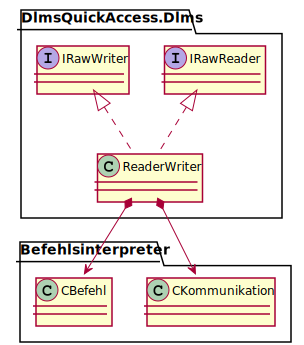
\includegraphics[width=0.5\textwidth]{gfx/dlms_vorher.png}
   \caption{
      Reduziertes Klassendiagramm um die ReaderWriter Klasse vor der Dependency Inversion
   }
   \label{fig:dlms_vorher}
\end{figure}

Da in diesem Sprint Änderungen am Kommunikationscode, also an DlmsQuickAccess.Dlms, geplant sind, wurde als erstes die zuvor gennante Koplung bereinigt.
Dazu wurde das Dependency Inversion Principle angewendet.
Dieses besagt, dass High-Level-Module nicht von Low-Level-Modulen abhängen sollen.
Beide sollten von Abstraktionen abhänig sein \parencite{madasu35solid}.
Das Klassendiagramm in Abbildung \ref{fig:dlms_vorher} zeigt, wie die Klasse ReaderWriter von Klassen des Befehlsinterpreter abhänig ist.
Wie die Abhänigkeiten nach dem Refactoring nach Dependency Inversion Principle aussehen, ist in Abblidung \ref{fig:dlms_nachher} gezeigt.
Mit dem ICommunicator Interface definiert DlmsQuickAccess.Dlms nun lediglich die Schnistelle eines Objekts, welches vom ReaderWriter benötigt wird.
Dieses wird mit der Communicator Klasse implementiert. Eine Instaz dieser Klasse kann nun in den ReaderWriter injected werden.
Somit wurde die Koppelung von DlmsQuickAccess.Dlms und Befehlsinterpreter aufgelöst.

% evtl schreiben, wo Communicator instantiert wird



\begin{figure}[H]
   \centering
   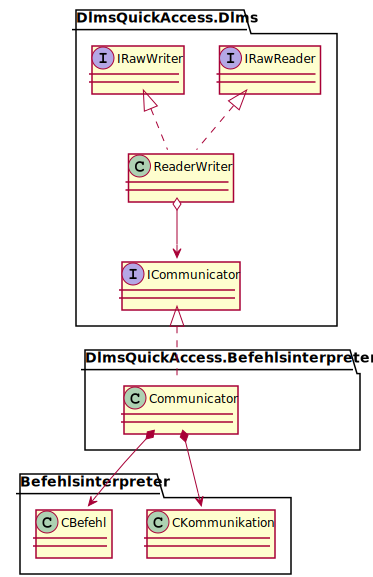
\includegraphics[width=0.5\textwidth]{gfx/dlms_nachher.png}
   \caption{
      Reduziertes Klassendiagramm um die ReaderWriter Klasse nach der Dependency Inversion
   }
   \label{fig:dlms_nachher}
\end{figure}

\subsection{states oder}

Kommunikation Asynchron machen
Bisher wird bei Kommunikation mit dem Zähler das UI eingefrohren
Wenn Kommunikation fehlschlägt stürtzt die Anwendung ab.
Kommt immer dan vor, wenn TLS Verbindung zuvor nicht sauber beendet wurde.

Die verschiedenen Zustände der Kommunikation soll mit dem State Pattern implementiert werden.
Das State Pattern ermöglicht, dass sich das Verhalten eines Objekts basierend auf dessen Zustand verändert \parencite{designPatterns}
Die Kommunikation kann mehrere Zustände haben:
\begin{itemize}
   \item Uninitiert
   \item Initiert
   \item Kommunizierend
   \item Fehlerzustand
\end{itemize}
Je nach Zustand muss sie anders auf neue Anfragen reagieren.
Ist sie beispielsweise noch uniniteiert, muss sie zuerst initiert werden, bevor die eigentliche Anfrage kommunizert werden kann.
Vom kommunizierenden Zustand ist es möglich, dass sie in einen Fehlerzustand gerät.
Um diesen zu verlassen muss erneut initiert werden.
Abblidung TODO zeigt auf, wie diese Zustände mithilfe des State Patterns implementiert wurden.

\subsection{async}
Bsp. ReadyState bekommt Read() befehl.
-> Startet Read via ICommunicator des contexts.
-> Sets Next state auf Communicating state

IsCommuncating state erwartet die antwort des Reads.
Beantwortet den das await des ursprünglichen callers.
setzt zurück auf ReadyState
-> kann jedoch auch ein stop erhalten während des warten
   -> antwortet await ebenfalls (mit exception)

Schwierigkeit -> 
ATS Code nutz intern System.CurrentThread.Name für das Session Management.
Das Desing der Applikation sieht jedoch vor, dass die Kommunikation in Tasks ausgelagert wird.
Dann ist der Thread Name jeweils ein andere, als wenn aus dem UI oder Main Thread zugegriffen wird.

Lösung "1"



\subsection{Bereinigung der internen Abhänigkeiten}
"Sync Namespaces" sehr hilfreich.


\subsection{Gruppen}

Wunsch Ronny M. : Import / Export 


\subsection{Feedback}
Chakrit: 
- Landingscreen ist leer, wenn zuvor noch kein Produkt gestartet wurde. // auch von christoph
   - Wo finde ich einen Browser? // Chistoph
- Version nicht sichtbar im Loadingscreen
- Version nicht sichtbar im Log
- Wenn er via Windows startet steht im Log ein fehler.
- Enter to search

Someone:
- Lesen von Arrays stimmt nicht richtig
   - repro: Object list lesen

\subsection{Class Descriptions}



Bug, dass app crasht, wenn Description nicht vorhanden

\subsection{SonarQube}\label{s6:sonar}
Im Abschnitt \ref{quality:sonar} wurde das Tool SonarQube erklärt und festgehalten, dass es von der Landis+Gyr als bevorzugtes Software-Qualitatssicherungstool evaluiert wurde.
Zum Zeitpunkt dieser Arbeit verfügte die Landis+Gyr noch über keine laufende Instanz von SonarQube.
Deshalb wurde eine solche lokal auf dem Rechner des Entwicklers aufgesetzt.
Dies hat den Nachteil, dass ein Aufbau, wie er in Abschnitt \ref{sonar:funktionsweise} beschrieben ist nicht möglich ist.
Anstelle des \ac{CI} Servers muss der Build jeweils manuell augeführt und an die lokale SonarQube Instanz übermittelt werden.
Für dieses Projekt stellt dies kein Problem dar, da nur ein einzelner Entwickler am Code arbeitet.



% dotnet sonarscanner begin /k:"DlmsQuickAccess_NoATS" /d:sonar.host.url="http://localhost:9000"  /d:sonar.login="8568d95955df20f319cd05320e41bc4c8dac02f3"
% dotnet build DlmsQuickAccess_NoWinUI.sln
% dotnet sonarscanner end /d:sonar.login="8568d95955df20f319cd05320e41bc4c8dac02f3"
\newpage